\section{Problem klasyfikacji}
Informacje zebrane w postaci zbiorów danych można poddać analizie, aby odnaleźć w nich pewne reguły pochodzące ze świata rzeczywistego. Celem automatyzacji tego procesu powstał odłam sztucznej inteligencji nazywany uczeniem maszynowym. Polega on na tym, że komputer uczy się zbiorów danych i wykrywa w nich zależności, które wykorzystuje do przewidywania wyników. Dane mogą być w różnej postaci. W owej pracy wykorzystywane jest uczenie nadzorowane, czyli każda z próbek (jedna instancja danych) ma przypisane rozwiązanie. Nauka to proces polegający na dostrajaniu wybranego algorytu, któremu przekazywane są dane treningowe będące wydzieloną częścią zbioru poddawanego analizie. Po przeanalizowaniu przekazanych na wejście informacji algorytm porównuje wydedukowany przez siebie wynik z tym dołączonym do badanej próbki. W przypadku gdy odpowie błędnie poprawia on swoje parametry w celu minimalizacji straty, czyli ilości błędnych predykcji. Po nauce modelowi przekazywany jest zbiór testowy również będący wydzieloną częścią oryginalnego zbioru danych. Chcemy osiągnąć jak najwyższą generalizację, czyli sytuację, gdy model popełnia mało błędów po podaniu mu próbek odbiegających od tych, na których został on nauczony. Klasyfikacja jest jednym z możliwych do uzyskania rodzaji odpowiedzi. Mamy z nią do czynienia, kiedy wejściu przyporządkowywana jest jedna ze skończonej liczby niepokrywających się grup. Dzieli się ona na dwie wersje - binarną, gdy istnieją tylko dwie klasy decyzyjne, np. pies lub kot; oraz wieloklasową, gdzie wyników może być wiele, np. 5 stopniowe stadium choroby \cite{bishop2006pattern, classification_gov, classification_google}. 

Do zadań klasyfikacji moglibyśmy użyć prostego, łatwo interpretowalnego modelu, takiego jak drzewo decyzyjne albo regresja liniowa. Przy mało skomplikowanych danych owe rozwiązanie byłoby wystarczające, jednak w rzeczywistości często mamy do czynienia ze złożonymi problemami wymagającymi trudniejszych w użyciu, zrozumieniu czy stworzeniu rozwiązań. Random forest, XGBoost oraz sieci neuronowe są w stanie przeprowadzić precyzyjniejsze analizy i osiągać większą dokładność. Wiąże się to niestety z utratą ich przejrzystości i czytelności. Dzieje się tak, ponieważ starając się jak najlepiej przybliżyć korelacje zaistniałe pomiędzy cechami danych wejściowych, budują one olbrzymie struktury, które przez swoje gigantyczne rozmiary stają się nieczytelne dla człowieka prowadząc do braku jakiejkolwiek możliwości ich interpretacji bądź analizy \cite{ALI2023101805}. 

\begin{figure}[H]
    \centering
    
\includegraphics[width=0.75\linewidth]{Deep-Neural-Network-architecture.jpg}
    \caption{Przykładowa struktura sieci neuronowej \cite{dnn_conference_image}}
    \label{fig:example_of_dnn}
\end{figure}

Badacze, w celu określenia przejrzystości modeli, wprowadzili pojęcia różnokolorowych skrzynek. Należą do nich:
\begin{itemize}
    \item biała skrzynka (bądź też nazywana przezroczystą) – zaliczają się do niej prostsze modele uczenia maszynowego, które możemy zazwyczaj bez jakiejkolwiek pomocy bezproblemowo analizować spoglądając na ich strukturę, wyniki oraz parametry. Nie potrafią odwzorowywać skomplikowanych zależności, z tego powodu ich dokładność jest niska bądź średnia. Nie są one dostosowane do trudniejszych dziedzin, takich jak medycyna czy finanse.
    \item szara skrzynka – systemy będące pośrednim rozwiązaniem pomiędzy innymi pudełkami. Istnieje możliwość ich częsciowej interpretacji przy założeniu, że zostały starannie zaprojektowane. Do tej kategorii mogą się zaliczać, np. sieci bayesowskie. Mają lepszą jakość klasyfikacji niż poprzedni przypadek. Dzieje się tak ponieważ są bardziej rozbudowane, co zarazem przekłada się na większe problemy z ich zrozumiem.
    \item czarna skrzynka – należą do niej głównie sztuczne sieci neuronowe, które ze względu na swoją znaczną złożoność są kompletnie nieczytelne. Tę sytuację obrazuje Rys. \ref{fig:example_of_dnn}. Mają wysoką dokładność, jednak nie jesteśmy w stanie, patrząc na ich strukturę, ocenić skąd ona wynika.
\end{itemize}	

 \begin{figure}[H]
     \centering
     
\includegraphics[width=1\linewidth]{colorful_boxes.jpg}
     \caption{Rysunek obrazujący podział modeli ze względu na ich przejrzystość \cite{ALI2023101805}}
     \label{fig:colorful_boxes}
 \end{figure}

Dochodzą do tego dwa często stosowane w kontekście XAI pojęcia - interpretowalność i wyjaśnialność. Pierwsze z nich dotyczy stopnia sposobności zrozumienia całokształtu działania. Drugie oznacza w jakim stopniu człowiek jest w stanie zrozumieć dlaczego model podjął akurat taką decyzję posiadając określone dane wejściowe. Jest to lokalna analiza względem konkretnego przypadku, zkłada m.in. pokazanie toku ,,myślowego'' algorytmu \cite{IBM_interpretability_explainability, molnar2025}.
 
Techniki XAI powstały, aby kosztem dokładności zwiększyć przejrzystość modeli, bądź odwrotnie – zwiększyć jakość klasyfikacji w zamian za możliwość ich częściowego zrozumienia. Zamieniają, więc one czarne oraz białe skrzynki w szare skrzynki, poświęcając większą wartość na tę, której systemowi brakuje. Celem takich zabiegów może być: 
\begin{itemize}
    \item zwiększenie poprawności modelu, poprzez możliwość przeanalizowania jego działania, przy czym znalezienia miejsc, w których model doszedł do błędnych związków, nietypowych rozwiązań wcześniej nam nieznanych, dyskryminował przypadki (klasy, grupy) rzadkie lub jego wnioskowanie pochodziło z błędu ludzkiego np. powstałego przy obróbce danych wejściowych, a następnie ich naprawa lub wyeksponowanie; 
    \item znalezienie inspiracji do przyszłych prac. Owe niekonwencjonalne sytuacje mogą nam dostarczyć wiedzę i pomysły, które moglibyśmy wykorzystać przy innych projektach;
    \item wytłumaczenie modelu i jego przewidywań;
    \item aby odkryć dlaczego dochodzi do danego wyniku \cite{molnar2025}.
\end{itemize}

\subsection{Metody oceny}
Mamy do dyspozycji wiele miar określających jakość uzyskanego w trakcie nauki modelu. Najpopularniejsze z nich użwywane w problemach klasyfikacji zostały zamieszczone w Tabeli \ref{tab:metrics_description}. Dodatkowo precyzję, \textit{recall} (czułość, specyficzność) oraz F1-score można w przypadku klasyfikacji wieloklasowej zagregować za pomocą średniej arytmetycznej bądź ważonej. Wagą średniej ważonej jest liczebność próbek danej klasy.  
\begin{xltabular}{\textwidth}{|c|>{\centering\arraybackslash}X|>{\centering\arraybackslash}X|}
\caption{Metryki, ich opisy i sposób obliczania \cite{zheng2015evaluating, f1_score_wikipedia}}
\label{tab:metrics_description}\\
\hline
Metryka & Opis & Sposób obliczania \\ \hline
\endfirsthead
ROC AUC & AUC (ang. \textit{area under the curve}), to powierzchnia pod krzywą ROC będącą wyznacznikiem jak zwiększyłaby się liczba poprawnych klasyfikacji pozwalając na więcej negatywnych klasyfikacji. AUC jest sposobem na reprezentację tej funkcji za pomocą jednej wartości.  & Krzywą ROC rysujemy poprzez punkty, których zmienną X jest wskaźnik wyników fałszywie dodatnich, a Y wskaźnik wyników prawdziwie dodatnich (czułość)  \\ \hline
Dokładność & Częstość prawidłowej klasyfikacji & Stosunek poprawnych predykcji do wszystkich predykcji\\ \hline
Precyzja & Mówi ile jednostek z przewidzianych jako dodatnie rzeczywiście zostało prawidłowo przydzielonych do tej grupy  & Stosunek próbek przewidzianych poprawnie jako dodatnie do wszystkich próbek sklasyfikowanych jako dodatnie \\ \hline
Czułość & Miara mówiąca o tym, jak często model poprawnie klasyfikowałby próbki jako dodatnie posiadając do dyspozycji wyłącznie próbki dodatnie & Stosunek próbek poprawnie zaklasyfikowanych jako dodatnie do wszystkich dodatnich próbek \\ \hline
Specyficzność & Miara mówiąca o tym, jak często model poprawnie klasyfikowałby próbki jako ujemne posiadając do dyspozycji wyłącznie próbki ujemne & Stosunek próbek poprawnie zaklasyfikowanych jako ujemne do wszystkich próbek ujemnych \\ \hline
F1-score & Łączy precyzję i czułość w jedną zbalansowaną wartość. & Średnia harmoniczna pomiędzy precyzją a czułością - dwukrotność precyzji pomnożonej przez czułość dzielona na sumę precyzji i czułości \\ \hline
\end{xltabular}


\subsection{Random Forest}

Random Forest, czyli las losowy, to metoda polegająca na zbieraniu wyników z wielu niezależnych modeli, aby na ich podstawie udzielić odpowiedzi końcowej. Wykorzystuje w tym celu drzewa decyzyjne, których przykładową strukturę przedstawiono na Rys. \ref{fig:decision_tree} Składają się one z:
\begin{itemize}
    \item korzenia (ang. root node) – początkowy węzeł reprezentujący cały zbiór danych wejściowych,
    \item węzłów (ang. decision node) – punktów, w których zachodzi podział danych ze względu na wybraną cechę,
    \item gałęzi – linii prowadzących od danego węzła do kolejnego,
    \item liści (ang. leaf node) – miano węzłów końcowych, tworzonych jeśli kryterium stopu zostało spełnione. Na podstawie podzbioru próbek, które do nich trafiły ustalają wyniki klasyfikacji, bądź regresji. 
\end{itemize}
\begin{figure}[H]
    \centering
    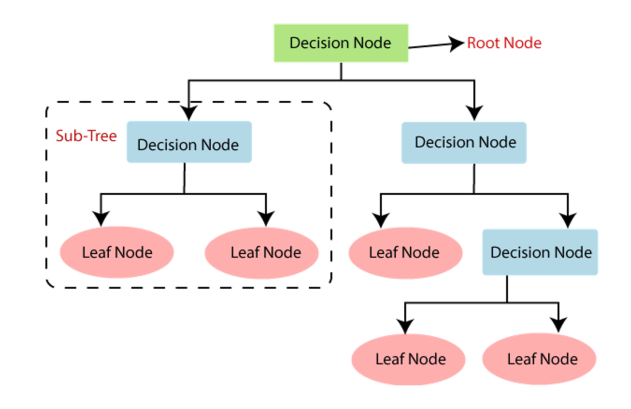
\includegraphics[width=0.75\linewidth]{rysunki/Decision-tree-illustration-Source.jpg}
    \caption{Struktura drzewa decyzyjnego \cite{decision_tree_image}}
    \label{fig:decision_tree}
\end{figure}

Budowę takiego lasu można określić jako rozszerzenie agregacji bootstrapowej – baggingu. Proces ten wykonuje się w celu redukcji wariancji i przeuczenia, co ma zwiększać dokładność i stabilność. Polega on na wygenerowaniu określonej liczby zestawów treningowych poprzez metodę bootstrap, czyli losowanie ze zwracaniem, niezależnym treningu podmodeli na tych nowych zbiorach, a następnie oszacowaniu wyników na podstawie ,,głosowania większościowego'' (problem klasyfikacji) lub średniej (w przypadku regresji). Rozszerzeniem będzie tutaj losowy dobór cech, który dokonuje się przy każdym podziale w drzewie. Powoduje to stworzenie modelu składającego się z nieskorelowanych drzew decyzyjnych.

Las losowy jest metodą charakteryzującą się wysoką dokładnością wyników, która potrafi poradzić sobie z obszernymi zbiorami danych a także występującymi w nich wartościami brakującymi. Niestety, z tego co zauważyłam, aktualnie nie jest w stanie przetworzyć zmiennych kategorycznych a duża ilość podmodeli sprawia, że jest ona trudna w interpretacji oraz może być czasochłonna i wymagać więcej zasobów sprzętowych, takich jak pamięć komputerowa \cite{molnar2025, random_forest_article, random_forest_cognity, bagging_definition}. 


\subsection{XGBoost}

XGBoost (ang. \textit{Extreme Gradient Boosting}) to metoda, która podobnie jak las losowy wykorzystuje wiele mniejszych modeli, w tym drzew decyzyjnych, aby określić wyniki. Jednak, w przeciwieństwie do poprzednio omawianego sposobu, działa na zasadzie boostingu, a nie baggingu. Proces ten polega na budowie sekwencyjnej. Każde drzewo (oprócz pierwszego) budowane jest na podstawie poprzednika dążąc do zmniejszenia ilości błędnych założeń. Początkowe podmodele są słabo przystosowane do problemu z mocą predykcyjną zbliżoną, ale lekko lepszą, niż losowe przydzielanie wartości, posiadają wysoki wskaźnik błędu. Mimo to są one niezwykle istotne ze względu na zawieranie kluczowych informacji dotyczących dzielenia zbiorów. Wraz z postępem algorytmu uczenia, czyli poprawą tych instancji oraz ich efektywnym połączeniem, wspomniane wcześniej miary zaczynają się polepszać. Kierunek, w którym ma poruszać się boosting, czyli tworzyć nowe drzewa, jest wyznaczany przez gradient. W tym przypadku oznacza ono pojęcie matematyczne odnoszące się do wektora składającego się z pochodnych cząstkowych funkcji. Wskazuje on kierunek, w którym najszybciej wzrasta wielkość funkcji w poszczególnych punktach \cite{gradient_definition}. 

Kolejną różnicą względem lasów losowych jest wielkość wspomnianych drzew. W przypadku tych pierwszych powstałe podmodele mogą osiągać duże rozmiary z wieloma odgałęzieniami. XGBoost charakteryzuje się niewielkimi instancjami, które są bardziej interpretowalne. Dodatkowo zawiera parametry wejściowe, które możemy dostosowywać, takie jak: liczba drzew, ilość iteracji, tempo uczenia, głębokość drzewa; a także mechanizmy regularyzacji w postaci L1 (ang. \textit{lasso regression}) oraz L2 (ang. \textit{ridge regression}) z możliwością zmiany ich współczynników. Należy zachować ostrożność w ich doborze, ponieważ to od nich zależeć będzie dokładność modelu, na którą żłoży się niedouczenie sieci, bądź jej nadmierne dopasowanie do danych treningowych. Może nam w tym pomóc walidacja krzyżowa, która jest zazwyczaj dostępna wraz z implementacją XGBoost’a.

Do zalet owej metody możemy zaliczyć możliwość użycia regularyzacji, wysoką dokładność, radzenie sobie z obszernymi zbiorami danych oraz pojawiającymi się w nich brakach, czy uczenie równoległe wykorzystujące wiele rdzeni CPU. Posiada ona jednak parę kluczowych problemów, takich jak: odpowiedni dobór parametrów, duże zużycie pamięci sprzętowej, trudności z przetwarzaniem danych kategorycznych, duży czas uczenia czy to, że przez swoje możliwości dostrajania jest mało przyjazna dla osób początkujących w dziedzinie sztucznej inteligencji \cite{xgboost_mamczur, xgboost_flowhunt, xgboost_analitycs_vidhya, xgboost_cognity, xgboost_pros_and_cons}. 

\subsection{Sieci neuronowe}

Sieć neuronowa to model nawiązujący budową do ludzkiego mózgu. Składa się z jednostek wzorowanych na neuronach, które są pomiędzy sobą połączone, co z kolei jest nawiązaniem do synaps. Elementy te układają się w kolumny tworząc warstwy. Pierwsza z nich, nazywana warstwą wejściową, ma liczbę neuronów odpowiadającą liczbie wejść (cech). Ostatnia warstwa - warstwa wyjściowa - zwraca wynik przewidywania. Składa się z tylu neuronów ile klas predykcyjnych została nauczona, zazwyczaj tyle do ilu mogą należeć wprowadzone dane. Warstwy pomiędzy tymi już omówionymi noszą miano ukrytych. Ich ilość oraz wielkość (liczba neuronów w poszczególnych kolumnach) zależy od twórcy \cite{rojas96neural}. 

\begin{figure}[H]
    \centering
    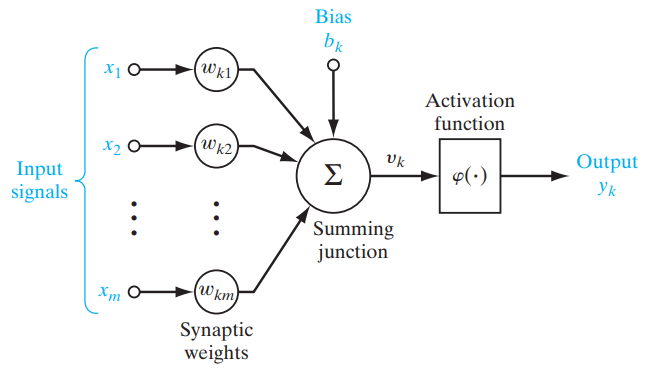
\includegraphics[width=0.75\linewidth]{rysunki/neuron_diagram.png}
    \caption{Model pojedynczego neuronu \cite{haykin2009neural}}
    \label{fig:neuron_diagram}
\end{figure}

Budowę pojedynczego neuronu przedstawia Rys. \ref{fig:neuron_diagram}, gdzie (idąc od lewej) wartości $x_1,\ x_2,\ \dots,\ x_m$ oznaczają kolejno $m$ wejść, $w_{k1},\ w_{k2},\ \dots,\ w_{km}$ to wagi dla każdego z $m$ wejść neuronu $k$, okrąg będący węzłem sumującym wejścia przemnożone przez odpowiadające im wagi i $b_k$, czyli bias neuronu $k$, który jest zewnętrzną wartością oddzielnie zwiększającą bądź zmniejszającą sumę (również posiada wagę). Następnie obliczona przez węzeł wartość oznaczona jako $v_k$ później przechodzi przez funkcję aktywacji $\phi(\ \cdot\ )$, która ocenia czy dany neuron na podstawie aktualnych danych powinien zostać pobudzony. W przedstawionym przeze mnie modelu każda z komórek może mieć połączenie jedynie z komórką z warstwy następnej, wyjatkiem jest ostatnia warstwa, w której budulce mają tylko jedno wyjście wychodzące na zewnątrz, nie mające połączenia z kolenymi elementami \cite{haykin2009neural}.

Nauka sieci neuronowej jest procesem mającym na celu wyznaczenie wag, które, jak wcześniej wspomniałam, są miarą istotności przekazywanych informacji. Jej najpopularniejszą metodą jest ,,uczenie w przód'' (ang. \textit{feedforward}). Odbywa się ona poprzez ustalenie wartości początkowych dla wag. Należy mieć na uwadze to, że nie powinny one być takie same, albowiem oznaczałoby to sytuację, w której wszystkie cechy przekazywałyby jednakowo istotną informację. Następnie na wejście modelu trafia pierwsza próbka z przekazanych danych treningowych będących wybranym (najczęściej losowo) podzbiorem naszego całego zbioru. Sieć równolegle wykonuje obliczenia na podanych informacjach. Wyjście neuronu staje się wejściem neuronu w następnej kolumnie o ile istnieje pomiędzy nimi połączenie. Wagi są poprawiane na podstawie wyliczanego błędu będącego chybieniem między przewidywaniem a wartością poprawną. Ruch odbywa się tutaj od lewej strony struktury (warstwy wejściowej) do prawej (warstwy wyjsciowej). Model przechodzi tak przez wszystkie próbki. Zmiana wartosci wag może odbywać się po przeanalizowaniu 1 przypadku lub zbioru przypadków nazywanego mini-batchem i nazywana jest iteracją \cite{dnn_architecture, haykin2009neural}.  

Stworzenie wydajnego modelu sieci neuronowej jest trudnym zadaniem. Do możliwych hiperparametrów, czyli parametrów ustalanych przed rozpoczęciem uczenia, należą:
\begin{itemize}
    \item liczba warstw ukrytych oraz ilość znajdujących się w nich neuronów, 
    \item dobór techniki uczenia, np. w przypadku uczenia przez wzmacnianie istnieje wiele rodzajów metod, takich jak Proximal Policy Optimization czy Deep Q-Network oraz ich modyfikacje;
    \item funkcje aktywacji, np. liniowa, ReLU, tanh; 
    \item algorytmy optymalizacji, polegające na minimalizacji funkcji straty,
    \item różne sposoby wyliczania funkcji straty (błędu w predykcji), np. ROC AUC i dokładność do zadań klasyfikacji oraz MAE, MSE, $R^2$ do regresji;
    \item ilość iteracji oraz wielkość zbioru, po którym następuje aktualizacja wag,
    \item krok uczenia.
\end{itemize}

Ich znalezienie odbywa się praktycznie na zasadzie ,,metody prób i błędów''. W doborze może nam pomóc mechnizm walidacji krzyżowej. Dodatkowo oceniając wyniki struktury z daną konfiguracją powinniśmy ustalić czy nie doszło do przeuczenia bądź niedouczenia. To pierwsze pojęcie oznacza sytuację, w której sieć wykryła zbyt drobne korelacje pomiędzy cechami, co było skutkiem zbytniego wglądu w dane treningowe. Taki przypadek zauważamy po niskim błędzie na danych treningowych, ale wysokim na danych walidacyjnych. Z pomocą przychodzą nam tutaj metody regularyzacji, takie jak L1, L2 czy Drop-out. Druga możliwość odnosi się do utrzymujących się wysokich błędów w przypadku obu podzbiorów. Polega na tym, że model nie zdążył wykryć zależności pomiędzy cechami, co przekłada się dodatkowo na jego niską dokładność. Dochodzi do tego, kiedy ustawiliśmy za małą ilość iteracji, za duży krok uczenia, bądź niewystarczająca ilość warstw ukrytych lub ich neuronów \cite{dnn_osowski, haykin2009neural, mlpc_documentation}. 

Kolejnym typem sieci wielowarstwowej użwanej w mojej pracy jest konwolucyjna sieć neuronowa (ang. \textit{Convolutional Neural Network}). Ta odmiana pozwala na analizowanie danych w postaci zdjęć. Na wejście takiej architektury podaje się obraz w postaci tensora - jednostki, którą w tym przypadku można sobie wyobrazić jako wektor składający się z 3 macierzy, w którym każda z macierzy reprezentuje jeden z 3 kanałów RGB obrazu a jej wartości to piksele mówiące o natężeniu danego koloru. Obraz trafia do warstwy splotowej składającej się z dowolnej ilości filtrów. Filtry mogą posiadać maksymalnie tyle kanałów ile mają trafiające do nich dane, czyli dla obrazów o trzech kanałach filtry będa posiadały maksymalnie 3 kanały. Sieć przesuwa tutaj po tensorze predefiniowaną maską z czego każdym wynikiem z nałożenia na obraz maski jest 2-wymiarowa tablica, w której elementy to przemnożone przez odpowiednie pozycje maski piksle zsumowane ze sobą. W taki sposób z 3 kanałów uzyskiwany jest 1, a ilość użytych filtrów staje się nową głębokością obrazu (kanałami). Tę operację nazywamy konwolucją od czego też wywodzi się nazwa owego podgatunku sieci. Na każdym z takich wyników należy zastosowac funkcję aktywacji ReLU niwelującą wartości ujemne poprzez zamianę ich na 0. Tablice reprezentują częściowo pokrywające się obszary. Aby rozwikłać problem nadmiarowości wprowadza się po każdej warstwie splotowej warstwę próbkującą, mającą na celu zmniejszenie wymiarowości poprzez zagregowanie wyników dla powtarzających się cech. Następnie wynik tych warstw trafia do kolejnej warstwy splotowej gdzie cykl się powtarza. Wraz z przechodzeniem przez kolejne warstwy sieci maleje szerokość i wysokość analizowanych macierzy, jednak ilość filtrów rośnie. Prowadzi to do zmniejszenia wymiaru a zarazem bogatszej reprezentacji wykrytych cech. Macierze ostatniej warstwy konwolucyjnej są przekształcane w wektor i trafiają do standardowych już warstw składających się z omówionych wcześniej neuronów, które są w pełni połączone z wynikami warstwy poprzedniej. Ostatnia warstwa sieci posiada tyle neuronów ile jest klas decyzyjnych, a ich wyjściami jest prawdopodobieństwo przynależności \cite{dnn_architecture, cnn_osowski,haykin2009neural}.

Ja użyłam już gotowych sieci konwolucyjnych o wagach nauczonych na bazie danych ImageNet. Dostosowałam ich parametry za pomocą \textit{transfer learning}'u. Proces ten polega na zamrożeniu warstw już wytrenowanej sieci, której rolą będzie wybieranie cech na obrazie oraz zbudowaniu naokoło nich warstw dostosowujących nowopowstały model nadrzędny do danego zadania, w tym przypadku klasyfikacji \cite{tensorflow_transfer_learning}. 